\begin{figure}[ht]
\centering
\newcommand\dapgwidth{0.14}
\newcommand\dapgoffset{-3.2}
\captionsetup[subfigure]{oneside,margin={0cm,0cm}}
\subfloat[\texttt{Hammer}. ]{
\begin{tabular}{c}
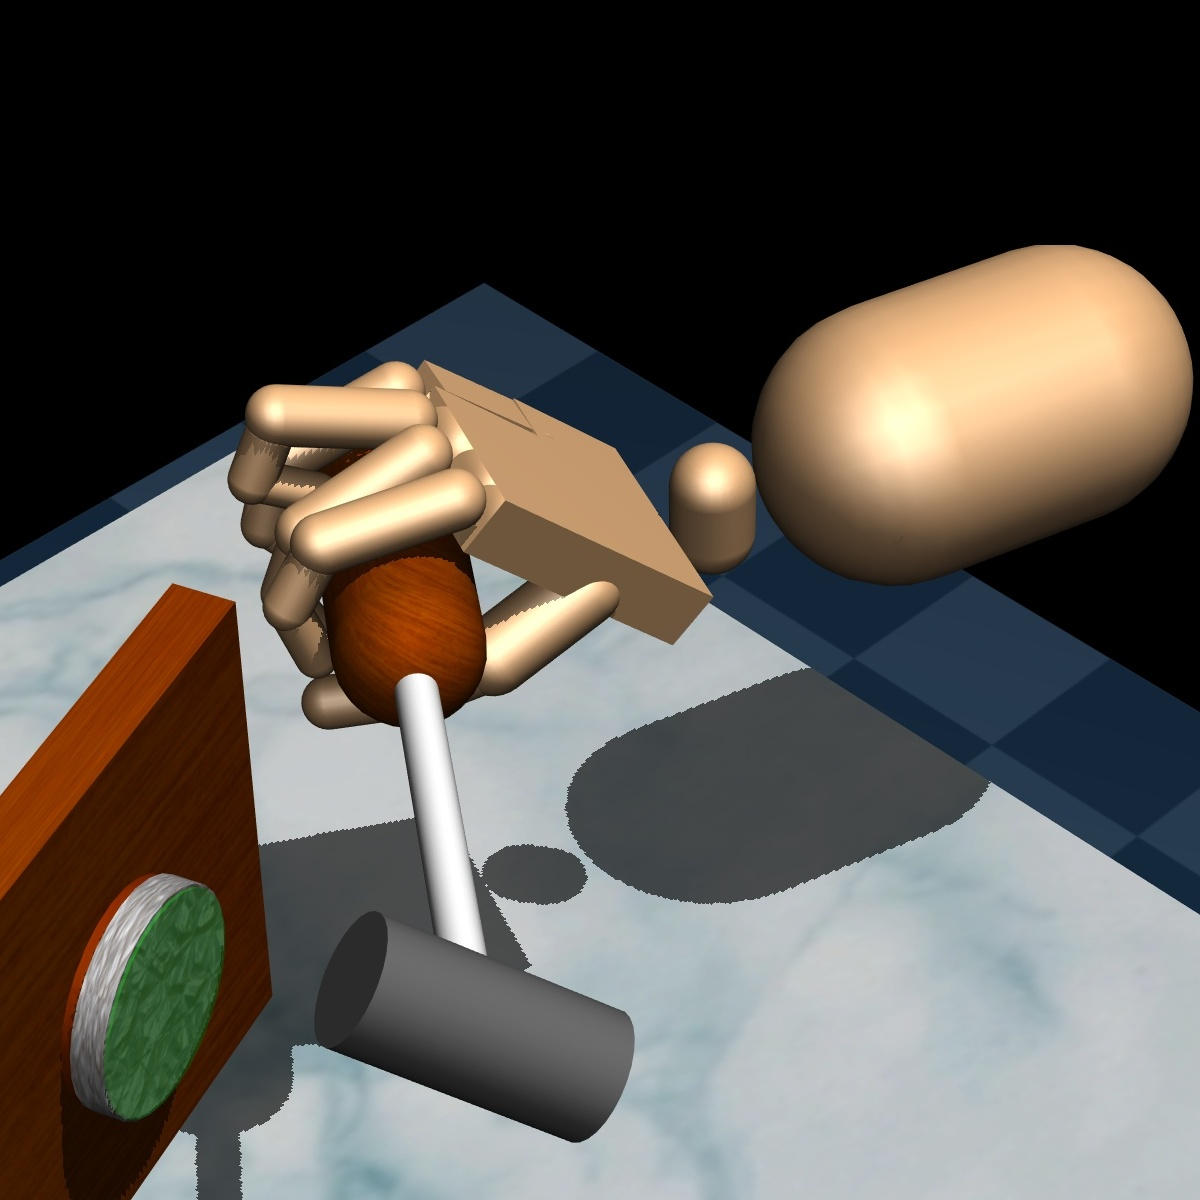
\includegraphics[width=\dapgwidth\textwidth]{Figures/dapg/hammer_0.jpg} \\
$\downarrow$ \\
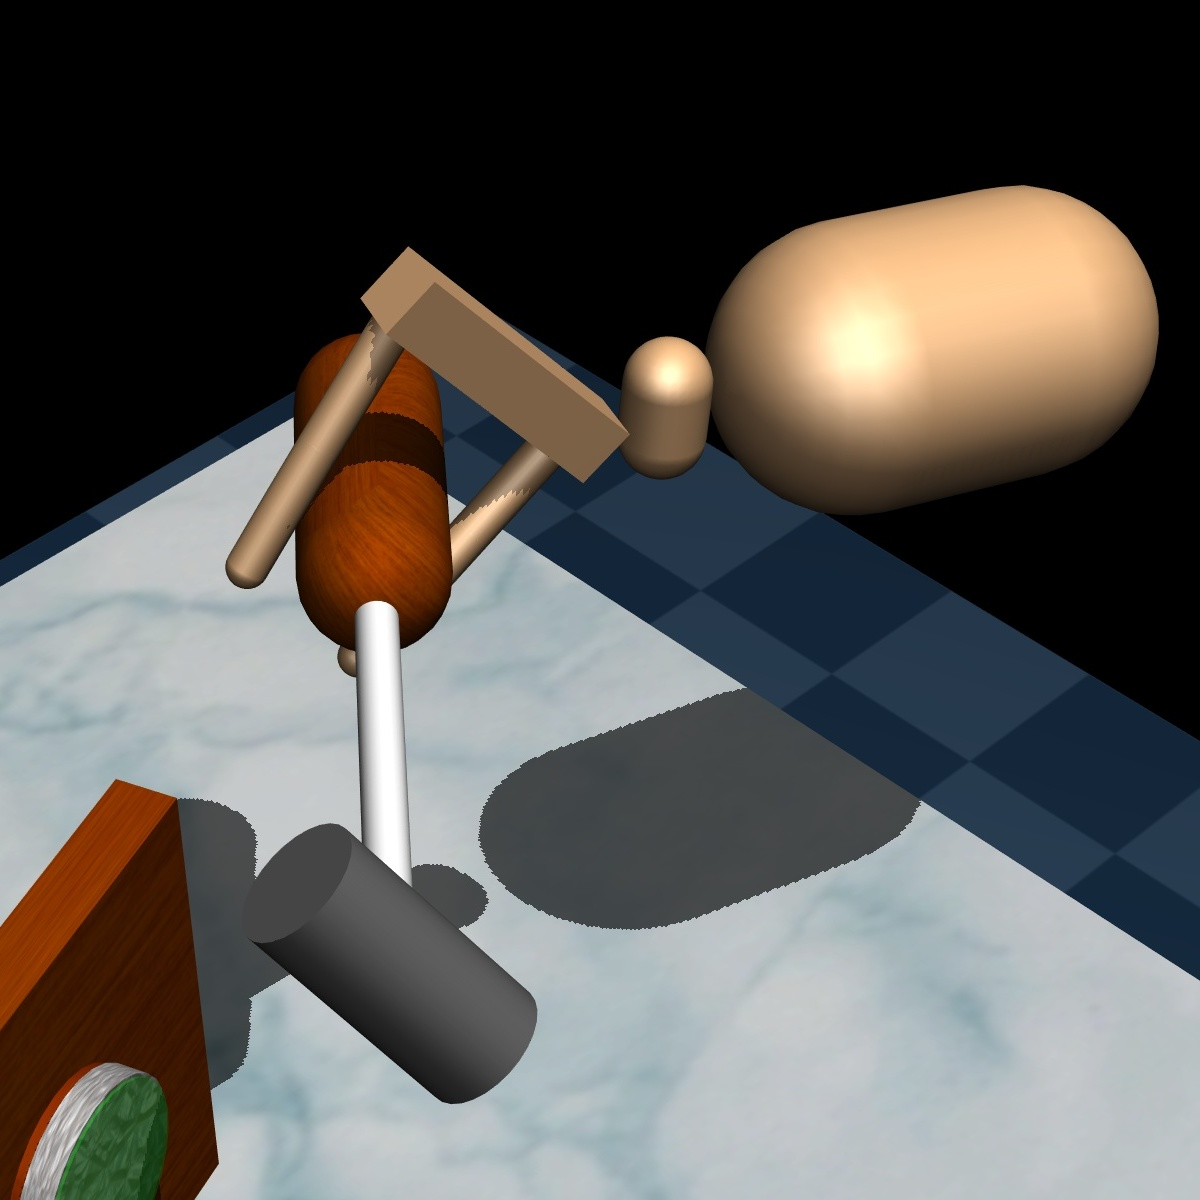
\includegraphics[width=\dapgwidth\textwidth]{Figures/dapg/hammer_1.jpg}
\end{tabular}
}
\hspace{\dapgoffset ex}
\subfloat[\texttt{Relocate}. ]{
\begin{tabular}{c}
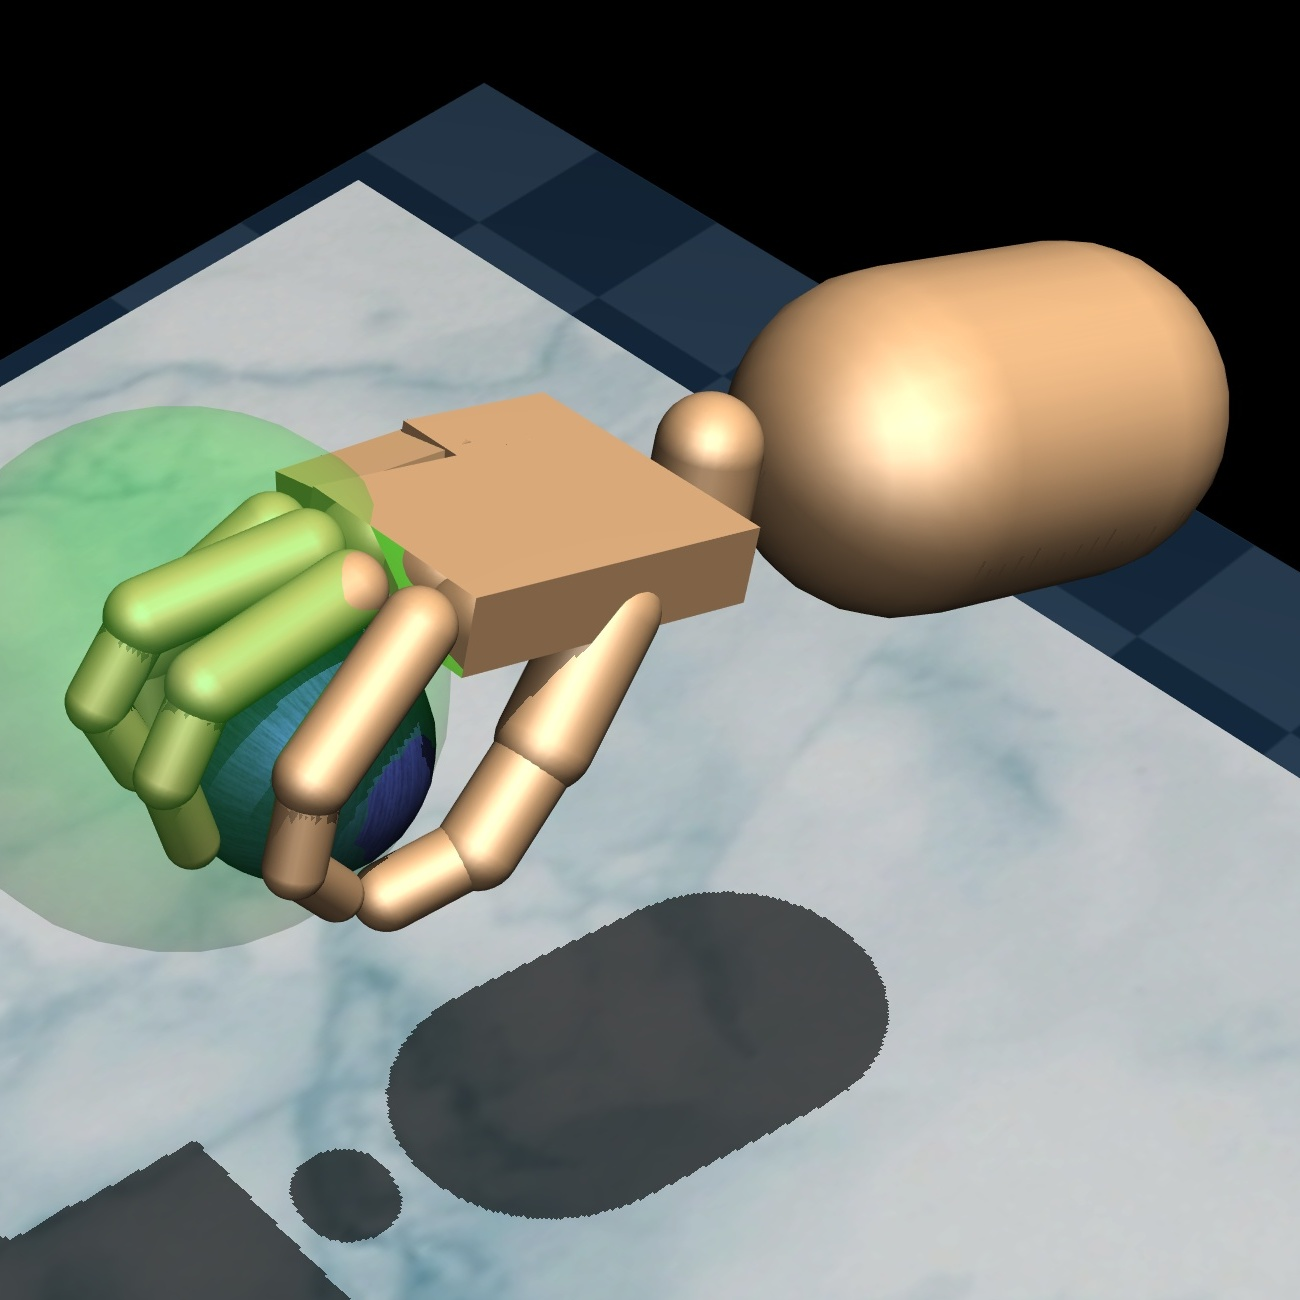
\includegraphics[width=\dapgwidth\textwidth]{Figures/dapg/relocate_0.jpg} \\
$\downarrow$ \\
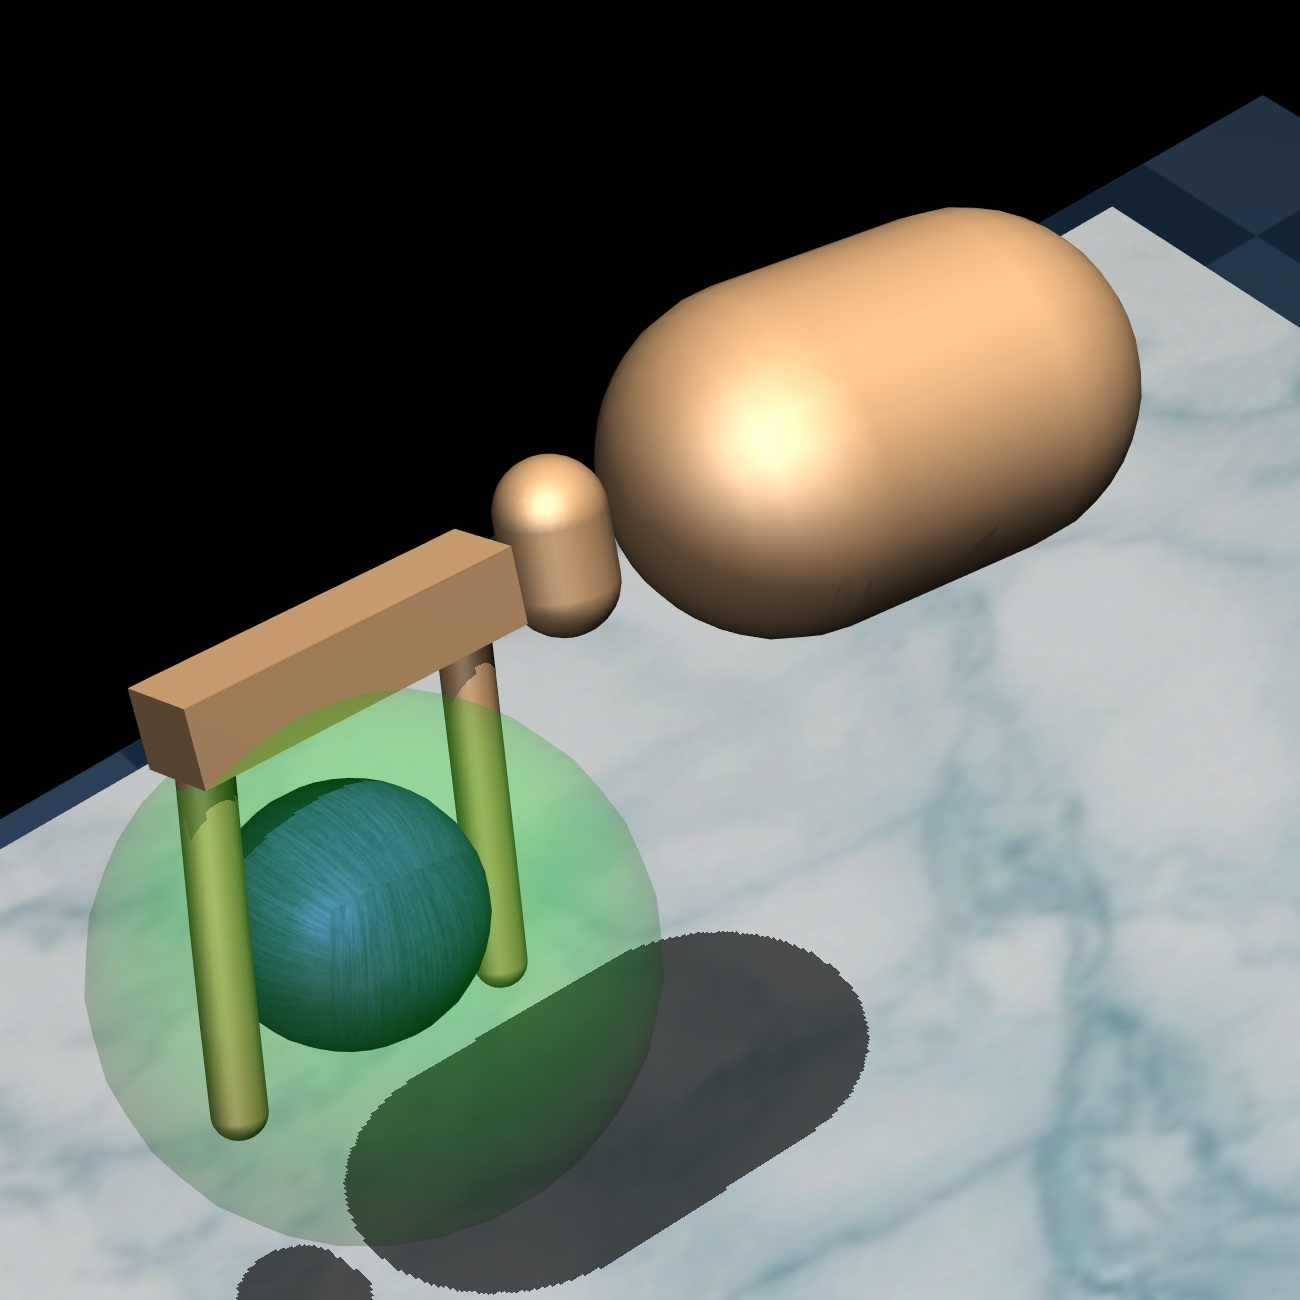
\includegraphics[width=\dapgwidth\textwidth]{Figures/dapg/relocate_1.jpg}
\end{tabular}
}
\hspace{\dapgoffset ex}
\subfloat[\texttt{Door}. ]{
\begin{tabular}{c}
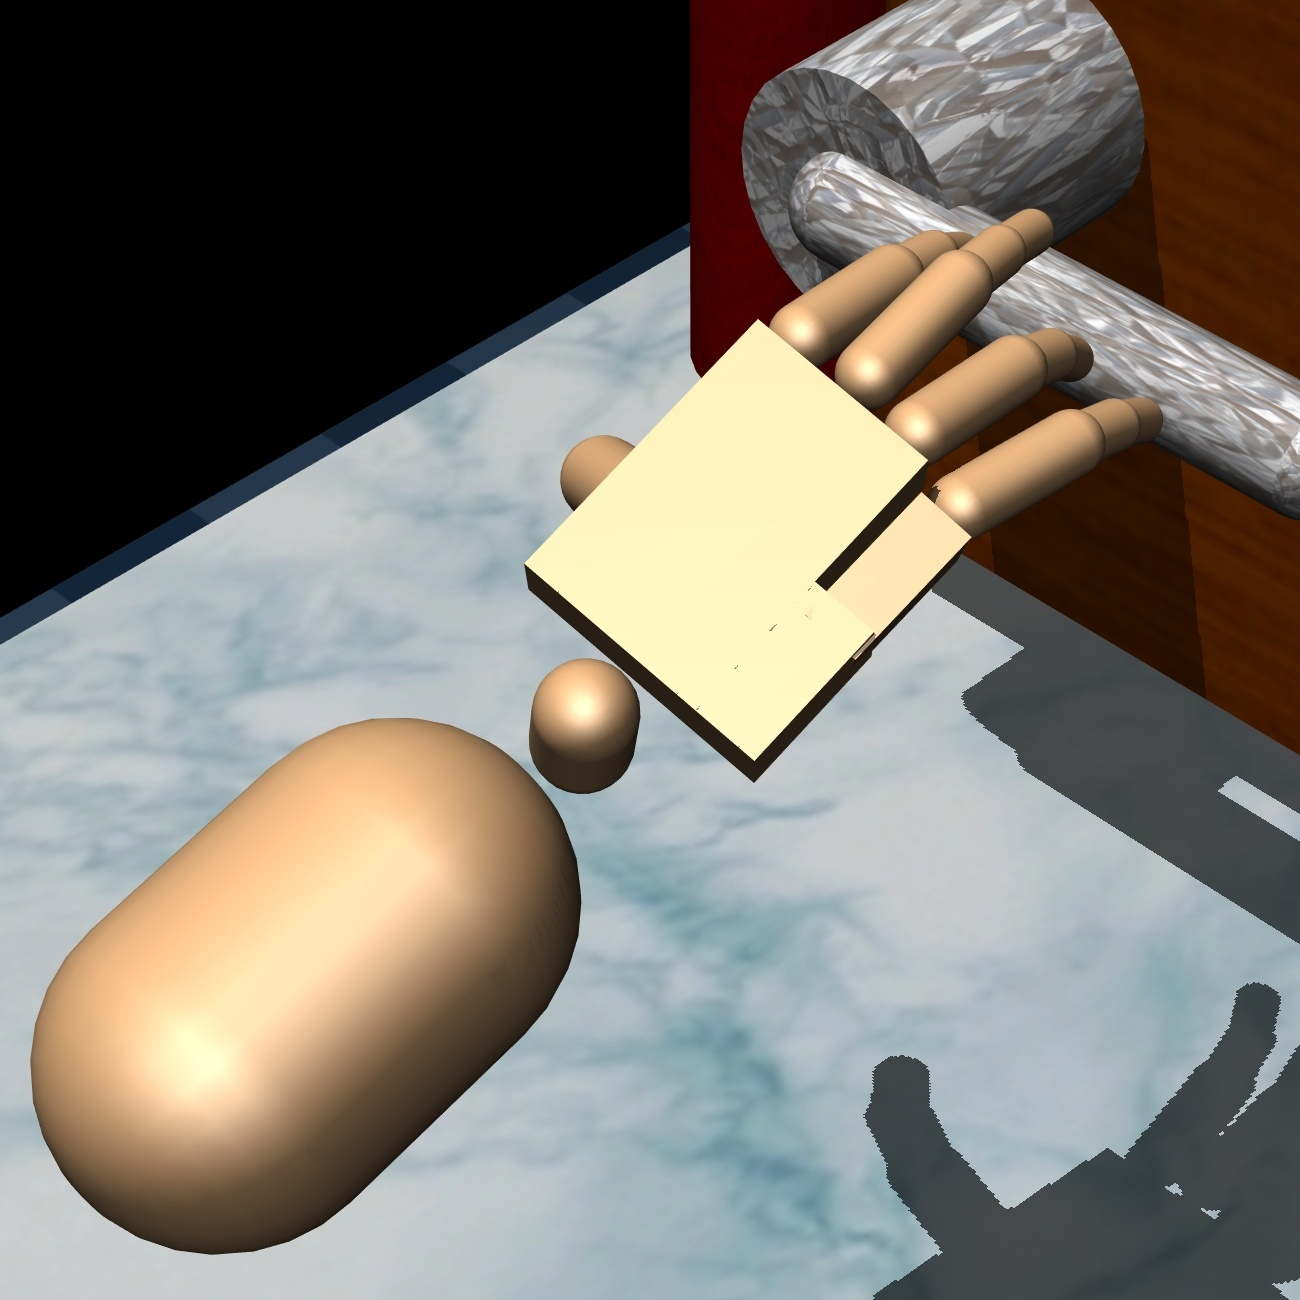
\includegraphics[width=\dapgwidth\textwidth]{Figures/dapg/door_0.jpg} \\
$\downarrow$ \\
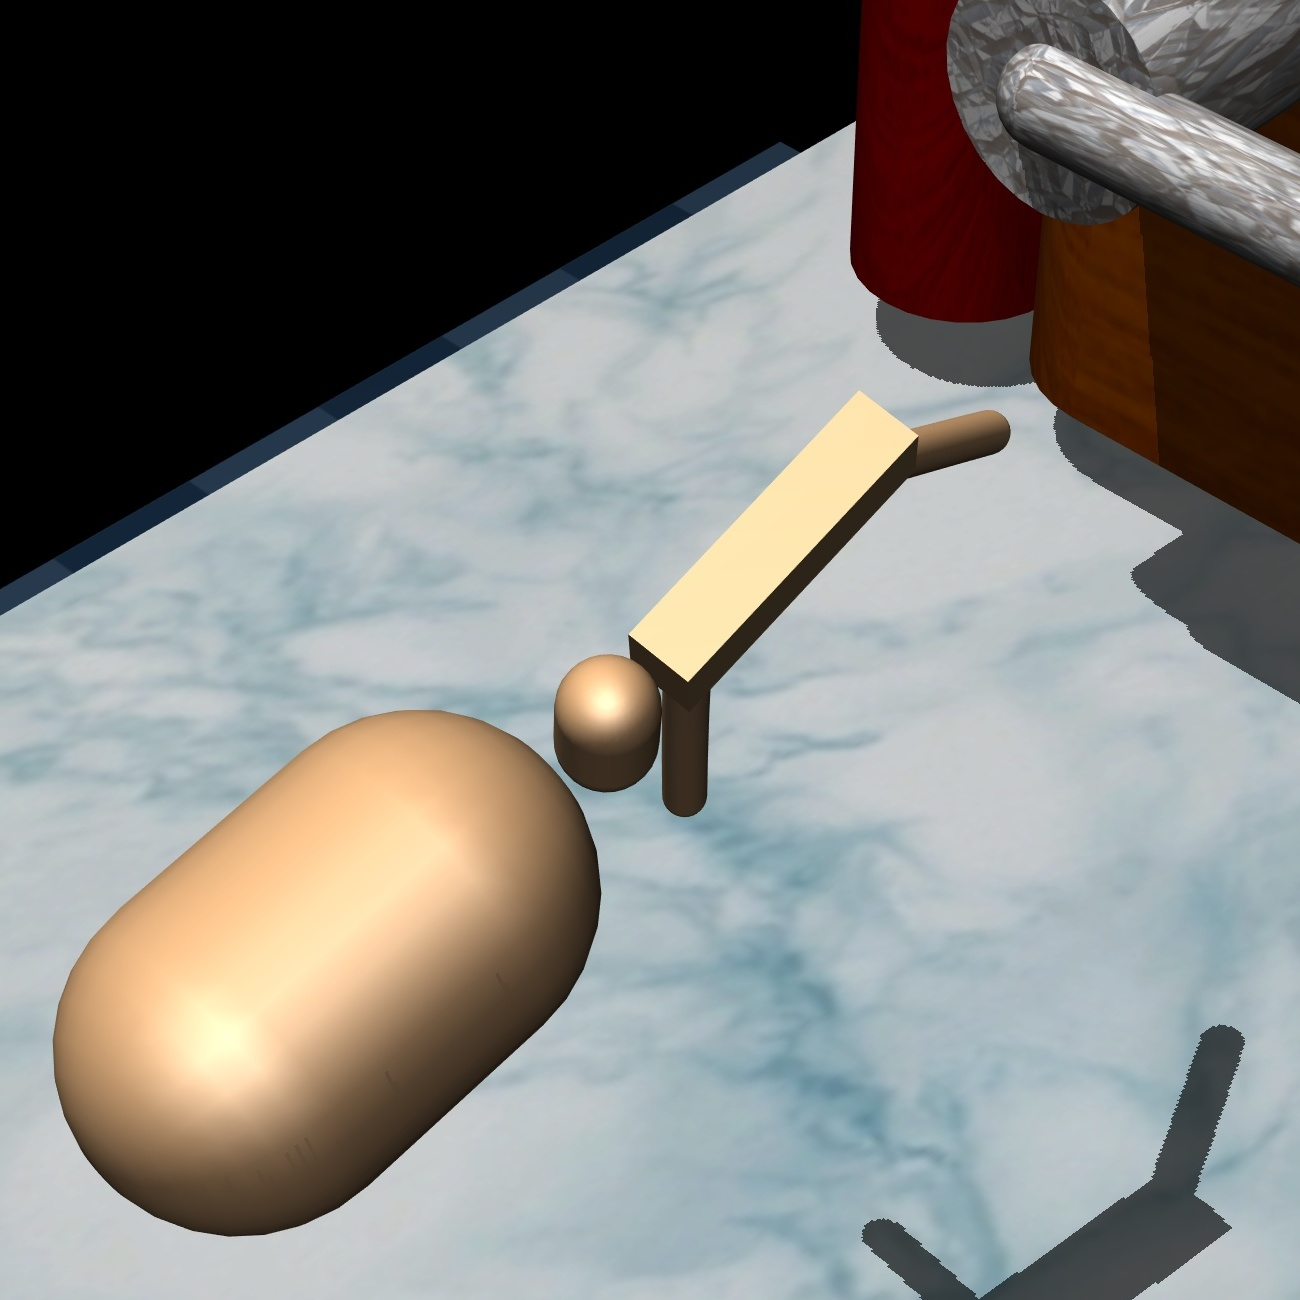
\includegraphics[width=\dapgwidth\textwidth]{Figures/dapg/door_1.jpg}
\end{tabular}
}
\vspace{-1ex}
\caption{\textbf{Hand Manipulation Suite tasks.}
(a) \texttt{Hammer} environment: the goal is to pick up the hammer and smash the nail into the board;
(b) \texttt{Relocate} environment: the goal is to pick up the blue ball and take it to the desired site shown by the green semitransparent sphere;
(c) \texttt{Door} environment: the goal is to switch the latch and fully open the door.
}
\label{fig:dapg}
\end{figure}

